%% Karlsruhe Institute of Technology
%% Institute for Anthropomatics and Robotics (IAR)
%% Artificial Intelligence for Language Technologies (AI4LT) lab
%%
%% Prof. Dr. Jan Niehues
%% Lab's website https://ai4lt.anthropomatik.kit.edu/english/index.php

\chapter{Evaluation}
\label{ch:Evaluation}
The evaluation of results of the experiments that were conducted on the benchmark section of the IWSLT 2023 dataset \cite{sperber2024evaluating} with regards to \autoref{ch:Dataset} as the relevant changes and preprocessing that was done.

The resulting scores are then pearson correlated \cite{2020SciPy-NMeth} to comet\footnote{the used comet implementation can be found here: https://github.com/Unbabel/COMET} scores as well as word error rates and compare those. The used pearson correlation implementation is the huggingface implementation \cite{huggingfacepearsonr}.

The comet scores are retrieved by using the regular translation from the MT models as well as the reference source transcription and the reference translation. 
These scores are used across all evaluation metrics in the MT category. 
%% -------------------
%% | Example content |
%% -------------------

\section{Transcription evaluation}
To evaluate how good the transcription quality estimation is the Word error rate\footnote{the used WER implementation can be found here: https://github.com/analyticsinmotion/werpy} \autoref{wer}, is used as reference score to compare the transcription quality estimation metric by correlating the WER scores with the help of the pearsoncorrelation \cite{2020SciPy-NMeth}
As WER is case sensitive, both the model result and the reference are normalised to be all lowercase, with single spaces, no leading or trailing blank spaces and no punctuation.
The resulting transcription probabilities plotted over the according WER values is shown in \autoref{fig:transcript scatter plot} and the pearson correlation can be found in \autoref{transcription results}. 
The plots in \autoref{fig:transcript scatter plot} demonstrate quite nicely the impact that normalizing the scores with the sequence length has, since \autoref{fig:transcript scatter plot base} shows less of a trend with the high model scores and low WER scores than \autoref{fig:transcript mean scatter plot}, which shows a more focused trend of higher WER scores and lower probability mean scores. 
However both methods show outlier values. For the transcription mean these are mostly low probability scores that have a low WER score as well, which means they are good transcripts. 
This also overlaps with the pearson correlation score, where the correlation score for the transcription mean is rounded 0.605 where as the non mean correlation score for the transcription probability is 0.331. 

This shows that taking the mean transcription probability is a good metric for estimating the transcription quality, as there are only a few outliers and a transcription probability mean score close to 0 means it is highly likely that the WER score will also be low. 

\begin{figure}[ht]
    \centering%
    \begin{subfigure}{0.45\linewidth}
        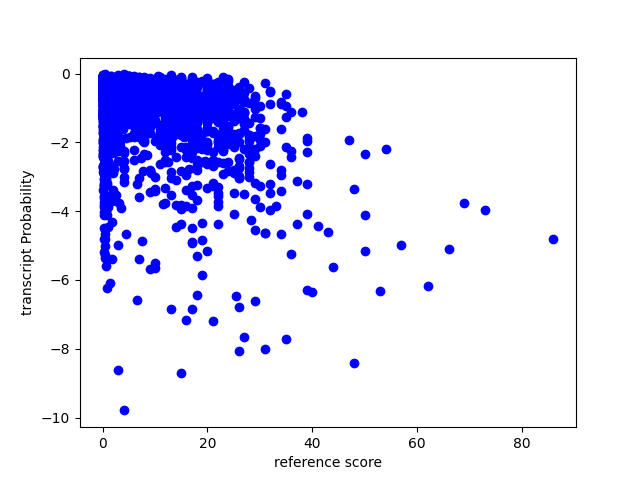
\includegraphics[width=\textwidth]{Latex/sections/images/transcriptbasescore.png}
        \caption{transcript scores over WER reference score}
        \label{fig:transcript scatter plot base}
    \end{subfigure}
    \begin{subfigure}{0.45\linewidth}
        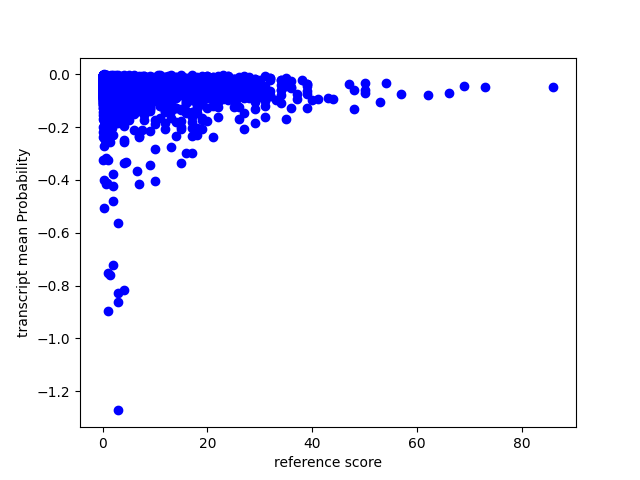
\includegraphics[width=\textwidth]{Latex/sections/images/transcriptmeanbasescore.png}
        \caption{transcript mean over WER reference score}
        \label{fig:transcript mean scatter plot}
    \end{subfigure}
    \caption{plot over the transcription probabilites, the transcription means and the WER scores}
    \label{fig:transcript scatter plot}
\end{figure}

\begin{table}[ht]
\centering%
  \begin{tabular}{l|d{2.6}}
  & \multicolumn{1}{l}{Whisper} \\ \hline
  Transcription Probability (-)& 0.33164 \\
  Transription mean (-)& 0.60496 \\ \hline
  Dropout transcription (-)& 0.2760 \\
  Dropout mean (-)& 0.3672 \\
  dropout variance &  0.1233\\
  dropout mean variance (-)& 0.0873\\
  dropout combo (-)& 0.1624\\
  dropout mean combo & 0.2684\\
  \end{tabular}

  \caption{result from the transcription part of the cascaded model, correlatated with WER scores, with the reference and model transcript normalized}
    \label{transcription results}
\end{table}

\section{Translation evaluation}
For the evaluation of the translation scores the reference score is genereated with the help of comet \cite{rei-etal-2020-comet}. This way of generating the reference score means that a score close to 1 is a good translation and a score close to 0 is a bad translation that is no better than random chance.
\begin{table}[ht]
\centering%
\begin{tabular}{l|d{2.6}d{2.6}d{2.6}}
&\multicolumn{1}{l}{Seamless}& \multicolumn{1}{l}{DeltaLM}&\multicolumn{1}{l}{Seamless e2e}\\ \hline
Translation & 0.37592 & 0.28284 & 0.656299\\ 
Softmax Entropy (-)& 0.30604&0.18071 & 0.60334 \\
Standard deviation (-)& 0.32905  & 0.25363& 0.67148 \\ \hline
Dropout translation & 0.150755& 0.282556& 0.14194\\
Dropout Variance (-)&-0.106986 & -0.16285& 0.13080\\
Dropout combo (-)& -0.163593& 0.179621& -0.20624\\ \hline
unified score$_{prod}$ (-)& 0.32965 & 0.05348 &\\
unfied score mean$_{prod}$(-)& -0.50055& 0.12587& \\
unified score$_{add}$&0.31837& 0.06600&\\
unified score mean$_{add}$&0.56032&0.168710&\\
\end{tabular}
\caption{Correlation scores for the separate models and calculated quality scores the sign on the left denotes weather the expected correlation value is supposed to positive or negative. If no signs are added to the values in a row then all of the values have the expected sign}
\label{results}
\end{table}
Those reference scores are then also pearson correlated with the scores from the model. The correlated scores for the translation part of the cascaded model and the speech translation part of the end-to-end model are found in \autoref{results}. 
As can be seen in \autoref{results} the scores retrieved from the model correlate well on the cascaded models with correlation scores of 0.376 for seamless and 0.283 for DeltaLm and really well on the end to end model with a correlation score of 0.656. 
The drop on the DelataLM model scores could be because of model differences with the seamless text-to-text translation model or due to the different score retrieval method, for this more experiments would have to be run with different models and the different toolkits. 
The drop could also be because even if seamless model used for text-to-text translation only uses text-to-text translation it might have learned different things during training that might help with translating, however this can be put down to model differences in the end. 
Another reason why the DeltaLm score on the translation probability is lower could be because it has more outliers with smaller translation proabilities but reference scores that are greater than 0.5, which can be seen in \autoref{fig:translationeval scatter plot translation}. However what can also be seen from the scatter plots is that DeltaLM has less low reference scores than seamless has. 
The end-to-end scores are that much higher, with 0.665 to 0.377 or 0.283, since there are no potential errors from the transcription part but it could also be that the model simply translates a lot better when using the seamless for spoken language translation. 
\todo{add plots for end to end?}

\begin{figure}[ht]
    \centering%
    \begin{subfigure}{0.4\linewidth}
        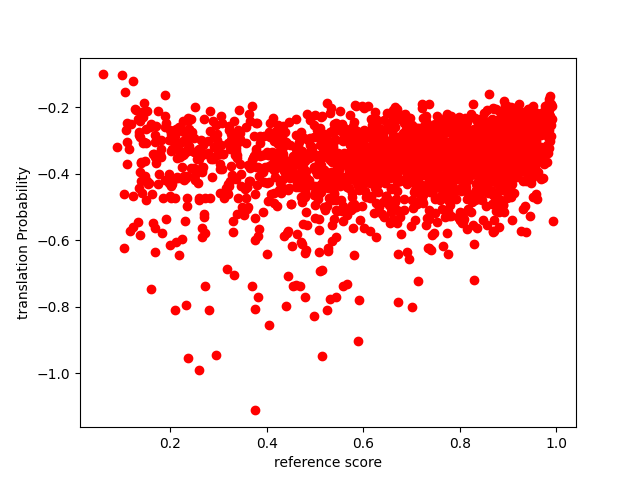
\includegraphics[width=\textwidth]{Latex/sections/images/seamlessgenprob.png}
        \caption{spread of the translation probability scores on seamless over the reference scores}
    \end{subfigure}
    \begin{subfigure}{0.4\linewidth}
        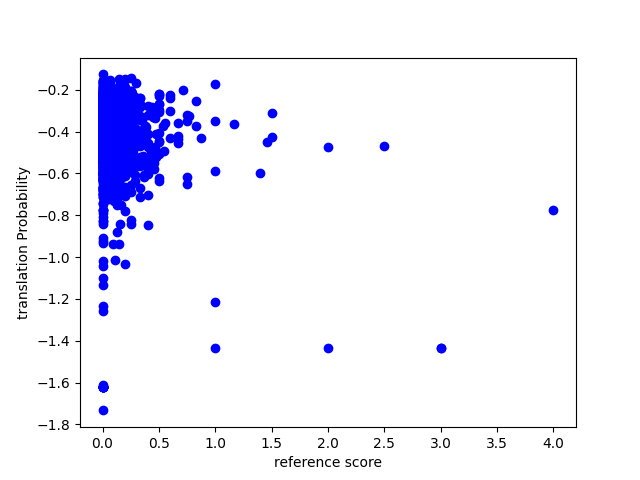
\includegraphics[width=\textwidth]{Latex/sections/images/dlmgenprob.png}
        \caption{spread of the translation probability scores on deltalm over the reference scores}
    \end{subfigure}
   \caption{Model translation scores over the corresponding comet scores. The left side shows the seamless scores, the right side shows the deltaLM scores}
    \label{fig:translationeval scatter plot translation}
    \end{figure}

The entropy scores anti-correlate with the reference scores, this is logical since the higher the entropy is the worse the translation. 
When looking at the absolute value of the correlation, so ignoring the sign, it can be seen that they correlate less with the references than the translation scores, as there is a 0.07 difference on seamless for text and 0.053 difference for end-to-end translation, as well as a 0.1 difference on DeltaLm, but they still correlate well with it, with correlation scores of 0.305 for t2t seamless, 0.180 for DeltaLM and 0.603 for e2e seamless.
The sofmax entropy scores plotted over the reference comet scores is shown in \autoref{fig:translationeval scatter plot entropy}, which also show quite well why the seamless pearson correlation scores are so much higher than the deltaLM correlation scores. This again might be because of the score retrieval method or it might be due to model differences. 
The end-to-end translation softmax entropy scores are once again higher than the text-to-text translation models this is most likely again due to less possible error from the transcription step.
\begin{figure}[ht]
        \centering%
    \begin{subfigure}{0.4\linewidth}
        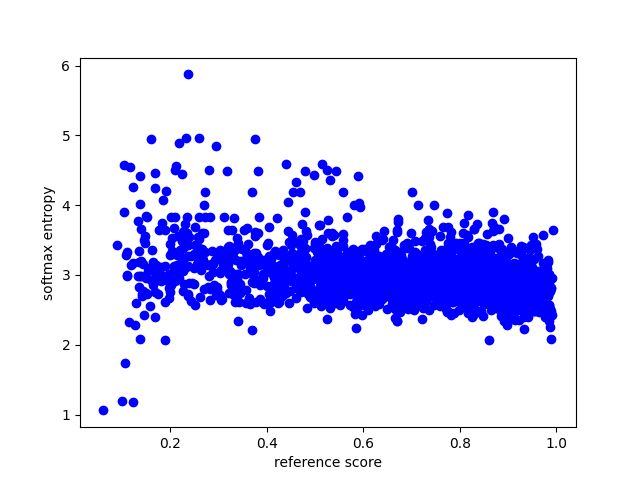
\includegraphics[width=\textwidth]{Latex/sections/images/seamlessentropy.png}
        \caption{seamless entropy scores over comet scores}
    \end{subfigure}
    \begin{subfigure}{0.4\linewidth}
        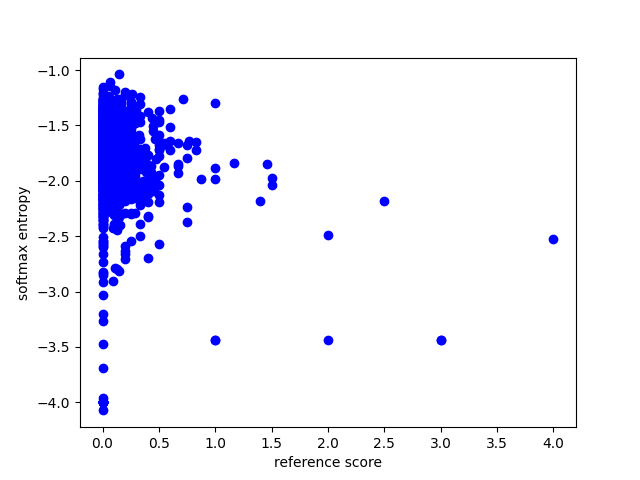
\includegraphics[width=\textwidth]{Latex/sections/images/dlmentropy.png}
        \caption{deltalm entropy scores over comet scores}
    \end{subfigure}
    \caption{Model softmax entropy scores over the corresponding comet scores. The left side shows the seamless scores, the right side shows the deltaLM scores}
    \label{fig:translationeval scatter plot entropy}
\end{figure}

The standard deviation scores, just like the Entropy scores anti-correlate, this is also due to how the standard deviation works as a lower standard deviation means less spread in the probabilities from the mean of those probability. 
Similarly to the softmax entropy, the absolute standard deviation correlation scores are also smaller than the translation scores but they correlate more to the reference scores than the entropy scores, with correlations scores of 0.329 for t2t seamless, 0.254 for deltaLM and 0.671.
Curiously enough the seamless end-to-end scores for the standard deviation have a higher correlation score than the translation score correlation with a correlation score of 0.671, which is most likely from the end-to-end nature of the model. Which means the model does not have to use an intermediate transcript and thus generating each top token can have different behaviour than the text to text models, it could also stem from the multilingual part of seamless. 
The standard deviation scores are plotted over the comet scores in \autoref{fig:translationeval scatter plot stddiv} which also shows well how the scores are anti-correlated and it also shows that the scores are very similar to how the regular translation probability scores are looking plotted. 
    \begin{figure}
            \centering%
            
    \begin{subfigure}{0.4\linewidth}
        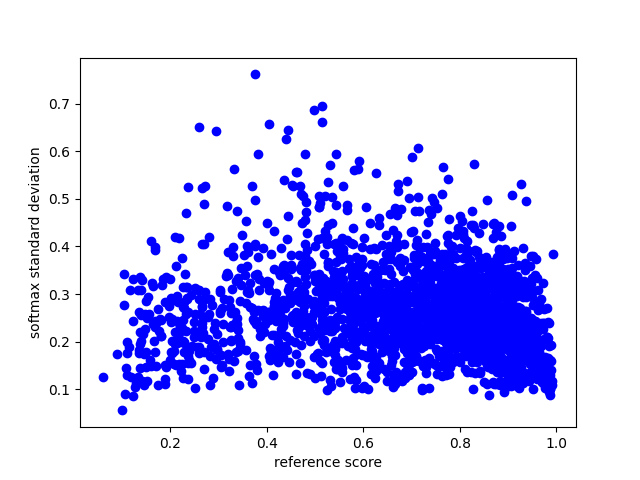
\includegraphics[width=\textwidth]{Latex/sections/images/seamlessstddiv.png}
        \caption{seamless standard deviation scores over comet scores}
    \end{subfigure}
    \begin{subfigure}{0.4\linewidth}
        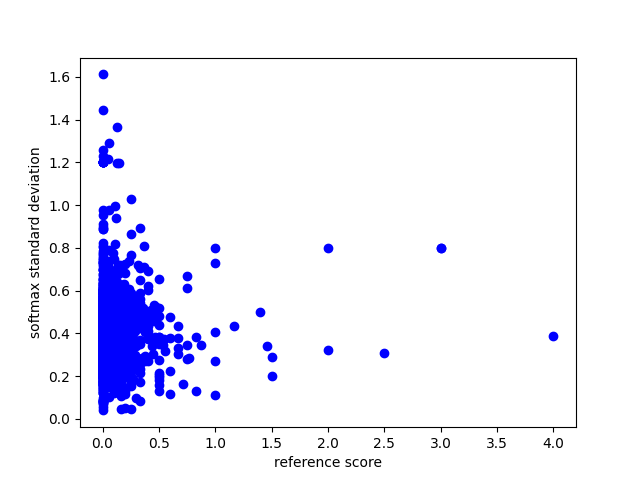
\includegraphics[width=\textwidth]{Latex/sections/images/dlmstddiv.png}
        \caption{deltaLM standard devation scores over comet scores}
    \end{subfigure}
    \caption{Model standard deviation scores over the corresponding comet scores. The left side shows the seamless scores, the right side shows the deltaLM scores}
    \label{fig:translationeval scatter plot stddiv}
\end{figure}

Based off of these results and possible error causes it can be gathered that the best metric for quality estimation in text and spoken language translation is the translation probability, this is both because it is easy to implement in most models and frameworks or toolkits, where it most of the time is already included and because it delivers good correlation results with reference scores, as explained above.
The next best metric would be the standard deviation of the decoding step probabilities, this is the case because it delivers good results in terms of correlation which might also have more potential for new scores on end-to-end models and because it is also fairly easy to implement, since getting the probability of the top token is what some toolkits or frameworks already allow and compiling the different scores during translation is also not difficult, then applying the standard deviation, which is part of any maths library is also simple. 
The worst method of these 3 methods would be the softmax entropy, because if the toolkit does not have it implemented already or a way to get the probability dirstibution over the vocabulary at each decoding step, it can be difficult to implement and it does not deliver scores that are better than any of the other scores proposed in this section. However the softmax entropy might be an interesting metric if used during dropout on text-to-text translation, more on that can be found in \autoref{dropout softmax entropy}.

\section{Dropout evaluation}
The dropout score is calculated by taking the mean of the dropout probabilities of the model, the variance of the dropout probabilities and a combination of both, the dropout score is then Pearson correlated with the comet scores or the word error scores in the case of the transcription. 
The reference scores are computed with the non dropout transcriptions and translations, since the dropped out sequences can differ a lot from the non-dropout sequences, which would impact the score and not accurately it represents the reference. 
The correlation results are listed in \autoref{results} for the translation part and \autoref{transcription results} for the transcription dropout. 

\autoref{fig:dropout transcript scores} shows the differences between the transcription probabilities and transcription mean in dropout. 
As can be seen if the scores are not normalized there is a lot less clear correlation between the low word error scores and high scores, as there are a lot more scores that have a low WER score but a broad spectrum of probability scores. This reflects in the correlation scores, the scores gathered with the mean of the transcription have a correlation score of 0.367 where the not normalised scores only have a correlation of 0.276. 
\begin{figure}[ht]
    \centering
    \begin{subfigure}{0.4\linewidth}
        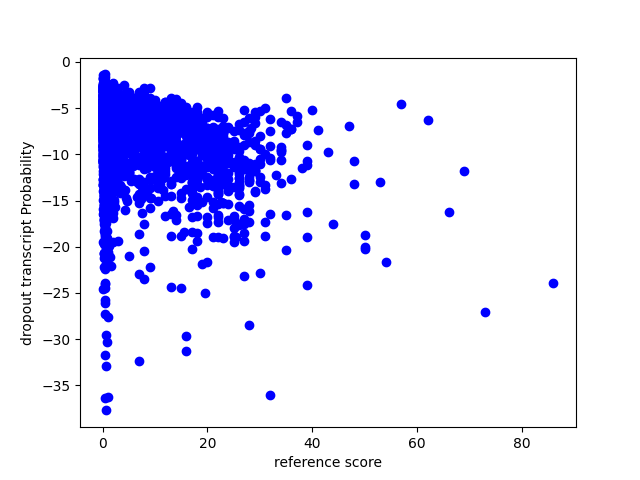
\includegraphics[width=\textwidth]{Latex/sections/images/seamlessdropouttranscript.png}
        \caption{dropout transcription probability scores over the reference scores}
    \end{subfigure}
    \begin{subfigure}{0.4\linewidth}
        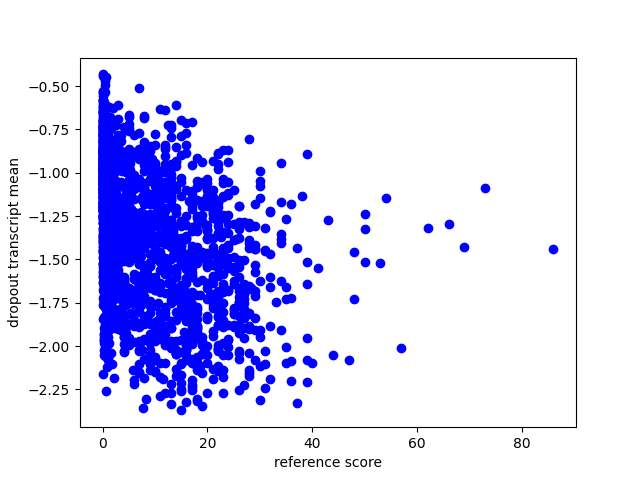
\includegraphics[width=\textwidth]{Latex/sections/images/seamlessdropouttranscriptmean.png}
        \caption{dropout transcription mean scores over the reference scores}
    \end{subfigure}
    \caption{transcription dropout scores plotted over the wer, left is the base scores, right half is the mean scores}
    \label{fig:dropout transcript scores}
    \end{figure}
    
The variance correltation is a lot higher in the non mean dropout with a correlation score of 0.123, than it is for the mean probability dropout with a score of 0.087, this is most due to a lot more variance in the length of the resulting transcripts and the impact of this variation in length on the score. The variance of the mean scores in dropout is a lot smaller this is most likely due to the normalisation and a resulting smaller impact on the scores. It should also be noted that the transcription mean variance correlation score is quite close to 0 and because of this not really statistically significant. a plot of these values can be found in \autoref{fig:dropout transcript variance scores} which also shows how not correlated the transcription mean dropout variance scores are to the WER. 
    \begin{figure}
        \centering%
    \begin{subfigure}{0.4\linewidth}
        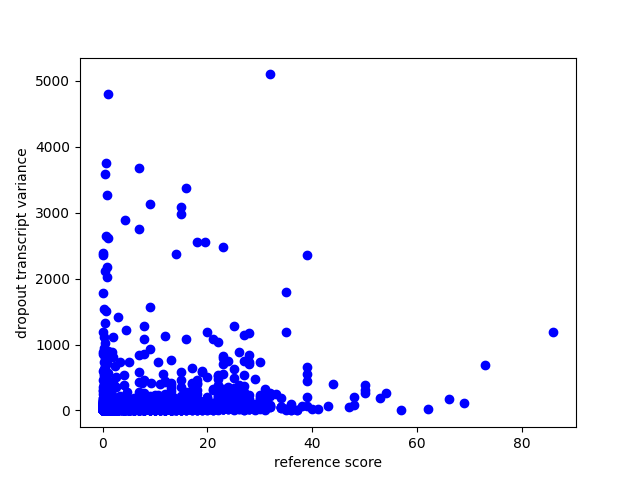
\includegraphics[width=\textwidth]{Latex/sections/images/seamlessdropouttranscriptvar.png}
        \caption{spread of the dropout transcription variance scores over the reference scores}
    \end{subfigure}
    \begin{subfigure}{0.4\linewidth}
        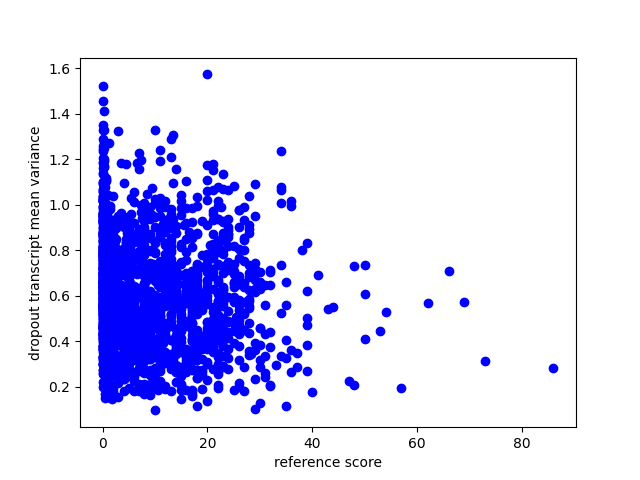
\includegraphics[width=\textwidth]{Latex/sections/images/seamlessdropouttranscriptmeanvar.png}
        \caption{spread of the dropout transcription mean variance scores over the reference scores}
    \end{subfigure}
    \caption{transcription dropout scores plotted over the wer, left is the base scores, right half is the mean scores}
    \label{fig:dropout transcript variance scores}
    \end{figure}
    
The combination score, which consists of the dropout transcription score and the dropout variance score, once again show decent correlation with the WER scores with correlation scores of 0.162 for the unnormalized scores and 0.268 for the normalised scores, which are lower than the dropout transcription score correlation by about 0.1 for each, but with how much lower the variance correlations are this is to be expected. The sign difference in the correlation scores comes most likely from the sign difference in the variance and the formula of how the combination score is calculated at each step as well as the fact that teh non normalized transcription variance scores are significantly higher than the variance values of the mean which leads to smaller values in the score. 
The plotted combo scores both for the transcription dropout scores and transcription mean dropout scores can found in \autoref{fig:dropout transcript combo scores}. They once again show that the mean displays a bit better distinction around the WER score of 0 than the transcription score. 
\begin{figure}
        \centering%
    \begin{subfigure}{0.4\linewidth}
        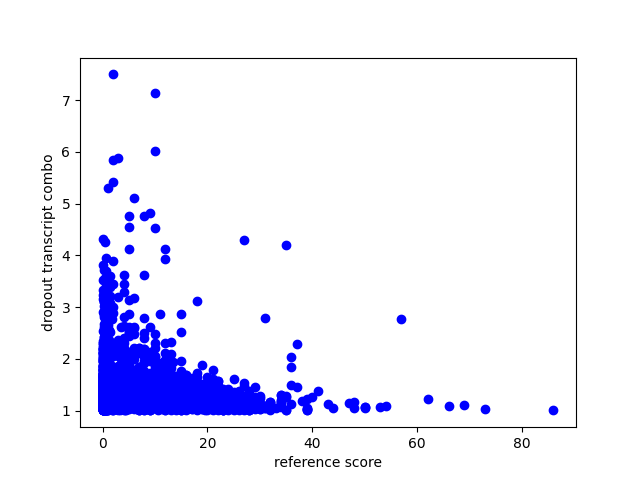
\includegraphics[width=\textwidth]{Latex/sections/images/seamlessdropouttranscriptcombo.png}
        \caption{spread of the dropout transcription combination scores over the reference scores}
    \end{subfigure}
    \begin{subfigure}{0.4\linewidth}
        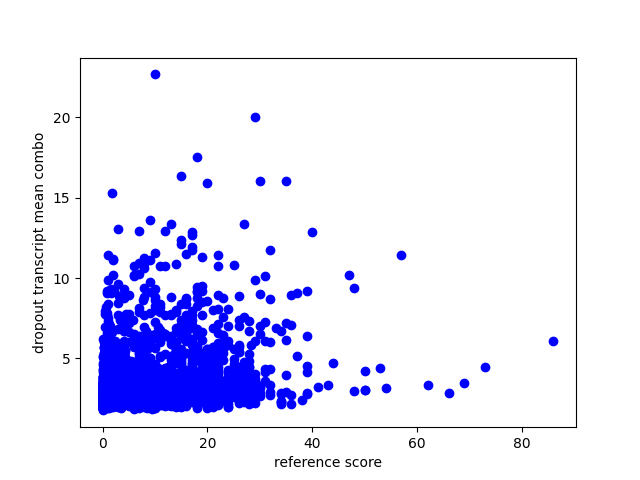
\includegraphics[width=\textwidth]{Latex/sections/images/seamlessdropouttranscriptmeancombo.png}
        \caption{spread of the dropout transcription mean combination scores over the reference scores}
    \end{subfigure}
    \caption{transcription dropout scores plotted over the wer, left is the base scores, right half is the mean scores}
    \label{fig:dropout transcript combo scores}
\end{figure}

%for this the dropout probabilities are calculated by running the model 30 times with the dropout layer enabled and then taking the mean and variance of the resulting probabilities. 
The baseline for the dropout is the dropout translation, found under that name in Table \autoref{results}, as can be seen the correlation between the seamless results, both the translation only with a score of 0.151 and the end to end versions with a correlation score of 0.142, is lower than the ones from DeltaLM which has a correlation score of 0.282, this is most likely due to how the dropout is implemented or used with the different toolsets/frameworks, but it could also be due to model differences. To properly distinguish between those possibilities more experiments would be needed where either dropout is enabled only on different parts of the model, so for example just the decoder, just the encoder, including attention and the like. Alternatively it might also stem from different versions of the input, into the dropout part of seamless but that would not explain the drastically lower score on the end to end version of seamless, since that takes the audio as an input. 
A plot of these scores can be seen in \autoref{fig:dropout translation probability scores}
\begin{figure}[ht]
    \centering%
    \begin{subfigure}{0.4\linewidth}
        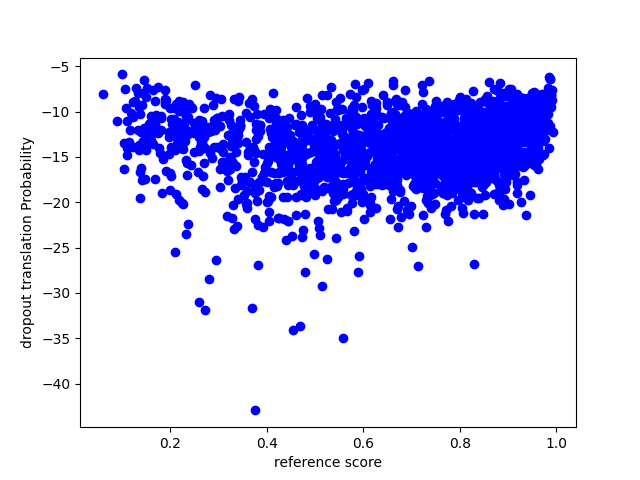
\includegraphics[width=\textwidth]{Latex/sections/images/seamlessdropprob.png}
        \caption{spread of the dropout translation probability scores over the reference scores for seamless}
    \end{subfigure}
    \begin{subfigure}{0.4\linewidth}
        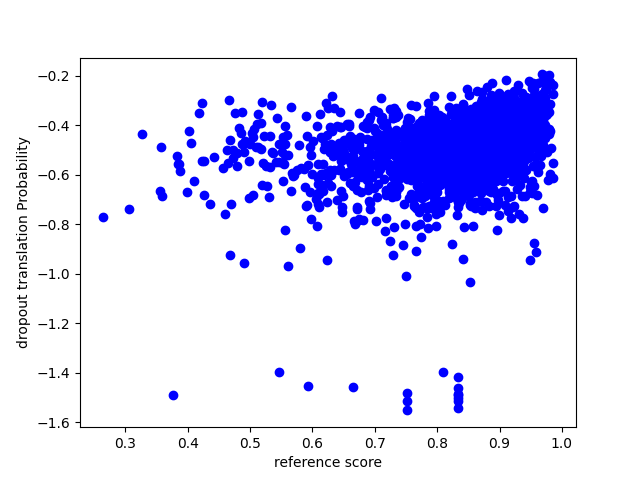
\includegraphics[width=\textwidth]{Latex/sections/images/dlmdropprob.png}
        \caption{spread of the dropout translation probability scores over the reference scores for deltalm}
    \end{subfigure}
        \caption{dropout probability scores plotted over the comet scores, left is the seamless scores, right half is the deltaLM scores}
        \label{fig:dropout translation probability scores}
    \end{figure}

The Variance scores are all smaller than the dropout probability scores, which as seen in the transcription part is to be expected, but while the pearson correlation of the translation dropout variance scores are smaller than the pearson correlation dropout translation probability score they are not that much smaller than them. The pearson correlation score can be found in \autoref{results} and a plot of the dropout variance scores over the reference scores can be seen in \autoref{fig:dropout translation variance score}.
The variance score is once again anti-correlated to the comet score, this is because of of how the variance works where a smaller score denotes a better result. 
The end-to-end dropout variance is not anti correlated, which can very well be due to a difference in reference score or can be a result of dropout.
As using dropout with the end-to-end model sometimes produces long stings of nonsense and because of how seamless is trained and what it can translate, those long strings do not always stick to a single language but rather switch through different ones and occasionally include characters from different alphabets. 
%An example of this can be found in \autoref{seamlesse2enonesense}
\begin{figure}[ht]
        \centering%
        \begin{subfigure}{0.4\linewidth}
        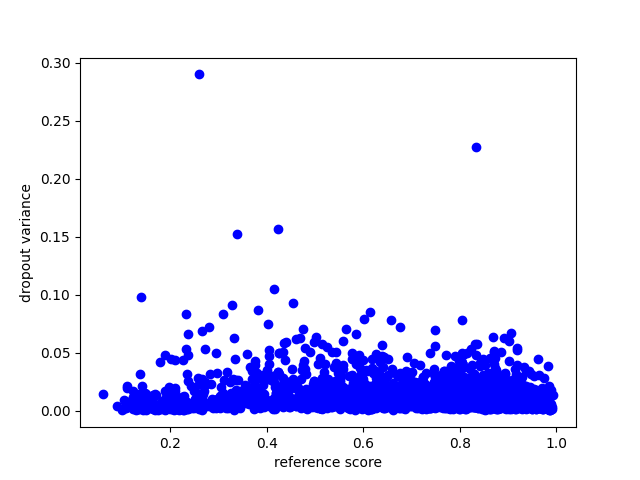
\includegraphics[width=\textwidth]{Latex/sections/images/seamlessdropoutvariance.png}
        \caption{spread of the dropout translation probability variance scores over the reference scores for seamless}
    \end{subfigure}
    \begin{subfigure}{0.4\linewidth}
        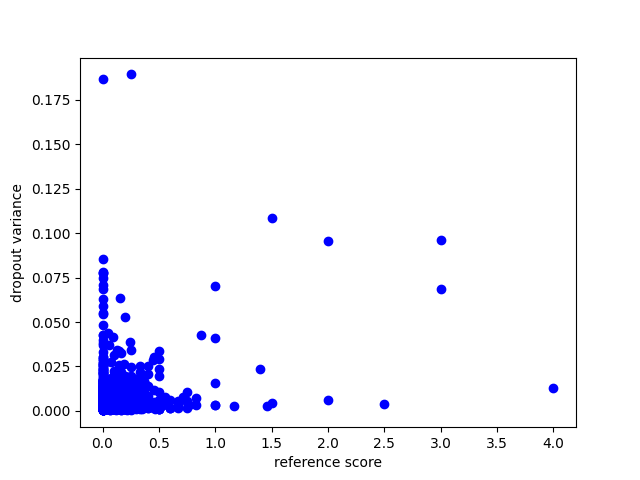
\includegraphics[width=\textwidth]{Latex/sections/images/dlmdropoutvariance.png}
        \caption{spread of the dropout translation probability variance scores over the reference scores for deltalm}
    \end{subfigure}
        \caption{dropout varinace scores plotted over the comet scores, left is the seamless scores, right half is the deltaLM scores}
        \label{fig:dropout translation variance score}
\end{figure}
    
The combination score made up out of the the other dropout scores show a stronger correlation with the reference scores than the variance but less than the translation probability for the cascaded models, with scores of -0.163 for seamless t2t and 0.180 for deltaLM, which considering how it is defines is to be expected. 
The flipped sign on the correlation score for deltaLM is most likely due to the incredibly small dropout variance scores and since the dropout translation score, which is negative, is divided by this variance score and then subtracted from 1.
However it is stronger correlated in the case of the end to end model with a correlation score of -0.206, this is most likely due to the correlation instead of anti correlation in the variance and the very similar correlation score between the dropout translation and dropout variance scores. 
The an overview over the pearson correlation scores again can be found in \autoref{results} and a plot of the scores for seamless t2t and deltaLM over the reference scores can be found in \autoref{fig:dropout translation combo}. 

\begin{figure}[ht]
        \centering%
    \begin{subfigure}{0.4\linewidth}
        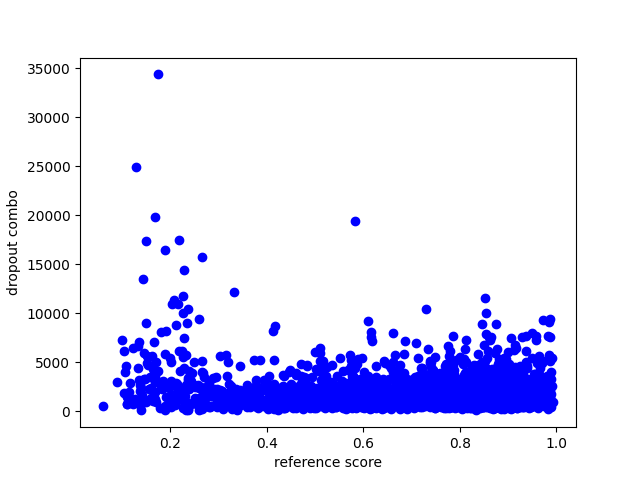
\includegraphics[width=\textwidth]{Latex/sections/images/seamlessdropoutcombo.png}
        \caption{spread of the dropout translation probability combo scores over the reference scores}
    \end{subfigure}
    \begin{subfigure}{0.4\linewidth}
        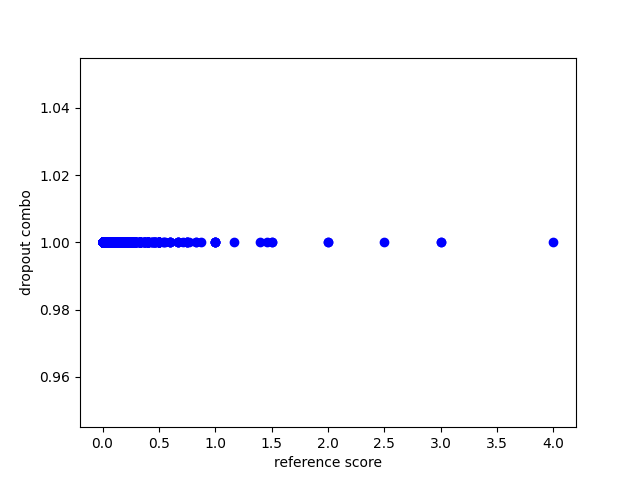
\includegraphics[width=\textwidth]{Latex/sections/images/dlmdropoutcombo.png}
        \caption{spread of the dropout translation probability combo scores over the reference scores}
    \end{subfigure}
    \caption{dropout combo scores plotted over the comet scores, left is the seamless scores, right half is the deltaLM scores}
    \label{fig:dropout translation combo}
\end{figure}
\todo{explain results more?}

\section{One unified score}
Since several different metrics are used in the translation part of the cascaded model it is interesting which one might be the best choice to use in a unified score, from the text translation paper \cite{fomicheva2020unsupervised} we can gather that different metrics work better for different language groups, as this thesis only tested on english to german translation no definite choice can be made without looking at other languages as well.


For a unified score the baselines, which are the translation and transcription probability, are multiplied. 
The resulting pearson score that can be found in \autoref{results} is calculated by correlating this unified score, product of translation probability and transcription probability, with the the comet score multiplied by the by the WER mapped to be from 0 to 1 by dividing all WER scores by the worst, so highest, WER score in the dataset, if finding the highest WER score for the dataset is not possible using 100 as a value is a decent option, as most WER scores are below that, and subtracting it from 1. 
This is can be described mathematically as 
$$reference = cometscore*(1-\frac{WER}{max(WER)})$$
which was choosen since the transcription probability is anti-correlated to the wer and since the best score of the WER is 0 that had to be taken into account as it ruled out just flat out dividing the comet score by the WER.

The correlated scores for the multiplion version of the uni score show that this works better with the scores from seamless which has a correlation score of 0.329 with the non normalized transcription scores and a score of 0.501 with the normalized scores. where as the unified scores calculated with the translation scores from deltalm are much lower with the unified score with non normalized transcription scores being only 0.053 correlated and the correlation being 0.126 if the normalized transcription scores are used. 

For the added together unified scores a very similar correlation scores are achived, however with the main difference that it is correlated instead of anti correlated for all of them. Seamless also again has the higher correlation scores with 0.328 for the not normalized transcription unified score and a correlation of 0.560 for the score that uses the length normalized  transcription score. Whereas DeltaLM has a correlation score of 0.066 for the non normalized score and a score of 0.169 for the normalized one, which is 0.04 higher than the multiplied score. 

Alternatively a unified score can be achieved by weighing the translation and transcription probabilities differently, which results in the formula $$unifiedscore_\alpha= \alpha TP_{transcript} + (1-\alpha)TP_{translation}.$$ 
As can be seen in \autoref{fig:uniscore correlation} changing the weight between the transcription and the translation scores has a noticeable impact on the correlation scores. 
This also shows that the weighing for cascaded models is at least partially model dependent, if not framework dependent, but using a high $\alpha$ seems to yield good results on the non-normalised uniscores in either case. 
For the normalised unified score the correlations seem to differ on what the best $\alpha$ value would be, for seamless it would be in the 0.3 to 0.4 range where as for deltaLM it is around 0.98. 

\begin{figure}[ht]
    \centering
    \begin{subfigure}{0.4\linewidth}
        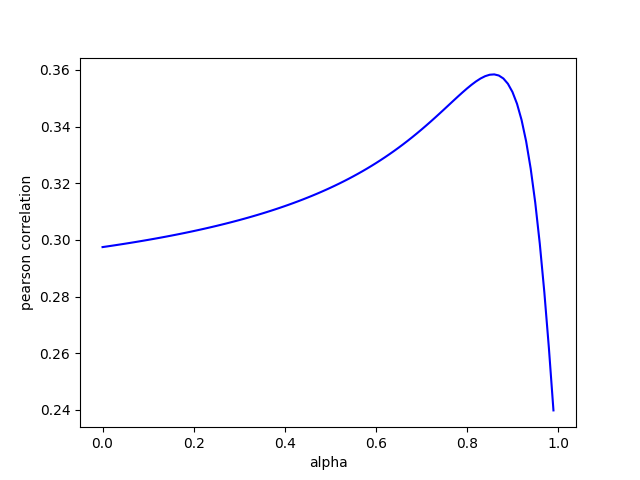
\includegraphics[width=\linewidth]{Latex/sections/images/seamlessuniscoredistribution.png}
        \caption{seamless unified scores}
    \end{subfigure}
    \begin{subfigure}{0.4\linewidth}
        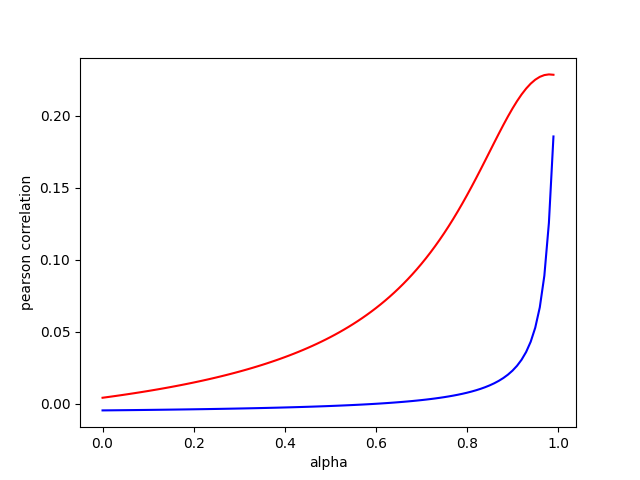
\includegraphics[width=\linewidth]{Latex/sections/images/dlmuniscoredistribution.png}
        \caption{deltaLM unified scores}
    \end{subfigure}
    
    \caption{Changes in correlation with different alpha values, the red line is for the unified score taken with the transcription mean, the blue line is the unified score gathered with the the non-normalised transcription score. }
    \label{fig:uniscore correlation}
\end{figure}

This shows that using the translation and length normalized transcription probabilities from cascaded models is a viable quality estimation, no matter if the translation and transcription scores are added together, multiplied or linearly interpolated for the score calculation. It also shows that finding the right weights for the transcription and translation parts can improve the correlation even more than simply adding or multiplying them together but to find out the right weights testing would have to be done as it seems to differ on a model basis.



